\documentclass{article}
\usepackage{amsmath}
\usepackage{tikz}
\usepackage{hyperref}
\usetikzlibrary{positioning}
\newcommand\abs[1]{\left|#1\right|}
\newcommand\floor[1]{\lfloor#1\rfloor}

\begin{document}

	\title{%
  	Introduction to Graph Theory \\
  		\large by Richard Trudeau \\
   		Ch. 5 Solutions}
   		\author{Tyler Bailey}
	\maketitle

	\begin{enumerate}

		\item[1] Draw all connected graphs that are regular of degree 1.
		
		\textbf{Solution}: There's just one connected graph of degree one: two vertices connected to each other.
		
		\item[2] Satisfy yourself that every connected graph which is regular of degree 2 is a cyclic graph. Show by example that deleting the word ``connected" results in a false statement.
		
		\textbf{Solution}: An example is a graph that has multiple disconnected cyclic graphs.
		
		\item[3] Verify that there is only one platonic graph with $v = 6$ and $e = 12$ (there are five of them) and checking that only the octahedron is platonic.
		
		\textbf{Solution}: I won't illustrate the graphs, but suffice to say it is probably easiest to check graphs whose complement has $v = 6$ and $e = 12$. In this way it is also easy to check that that there is only one graph whose complement can be regular.
		
		\item[4] Prove: there is no regular graph with $v = 6$ and $e = 10$.
		
		\textbf{Solution}: From Lemma 14, if $G$ is regular then $e = dv/2$, so we have $10 = 3d$ which obviously is not solvable for an integer $d$. Therefore $G$ is not regular.
		
		\item[5] Prove: if a graph has an odd number of vertices and is regular of degree $d$ then $d$ must be even.
		
		\textbf{Solution}: From Lemma 14, we have $e = dv/2$. If $d$ was odd then $dv/2$ would not be an integer, which is impossible. Therefore $d$ (if it exists... we have done nothing to prove that must be the case) must be even.
		
		\item[6] Find a graph other than the cube that has $v = 8$ and is of degree 3.
		
		\textbf{Solution}: Here is one such graph:
		
			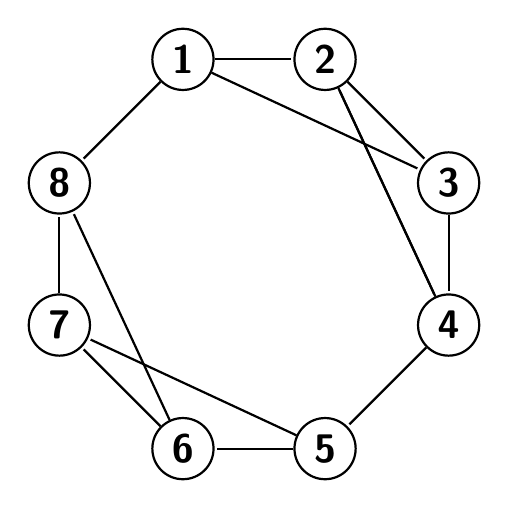
\begin{tikzpicture}[shorten >=1pt,auto,node distance=3cm, thick,main node/.style={circle,draw,font=\sffamily\Large\bfseries}]
				\node[main node] (1) {1};
				\node[main node] (2) [right=1cm of 1] {2};
				\node[main node] (3) [below right=1cm and 1cm of 2] {3};
				\node[main node] (4) [below=1cm of 3] {4};
				\node[main node] (5) [below left=1cm and 1cm of 4] {5};
				\node[main node] (6) [left=1cm of 5] {6};
				\node[main node] (7) [above left=1cm and 1cm of 6] {7};
				\node[main node] (8) [above=1cm of 7] {8};

				\path[every node/.style={font=\sffamily\small}]
					(1)	edge node [left] {} (2)
						edge node [left] {} (3)
						edge node [left] {} (8)
                		(2)	edge node [right] {} (3)
                			edge node [right] {} (4)
					(3)	edge node [right] {} (4)
                		(4)	edge node [right] {} (2)
                			edge node [right] {} (5)
					(5)	edge node [right] {} (6)
						edge node [right] {} (7)
					(6)	edge node [right] {} (7)
						edge node [right] {} (8)
					(7)	edge node [right] {} (8);

			\end{tikzpicture}
		\item[7] Omitted for size.
		
		\item[8] Omitted... I don't want to rob you of the fun of this one :)
		
		\item[9] Prove that every wheel graph $W_v$ is isomorphic to its (unique) dual.
		
		\textbf{Solution}: The isomorphism is that the infinite face is the part of the graph where all the spokes radiate from, and the dual vertices of inner faces are the outer rim of the wheel.
	\end{enumerate}

\end{document}